%!TEX root = ../../../super_main.tex

\section{Profile Selector Dialog}
\label{sec:profile_selector_dialog}

As mentioned in \secrefpage{sec:category_tool_and_components}, the \ct should be able to manage categories for the profiles, for this reason we need to be able to select multiple profiles using a dialog. In the shared components there was previous a profile selector called \androidinline{GProfileSelector} as seen in \figref{fig:puha_dialog}, however this type of selector does not allow for multiple selection of profiles. Furthermore, this selector was not consistent with the design of the new \gc, and it was therefore decided that a new selector should be implemented.

\begin{figure}[!htbp]
        \centering
        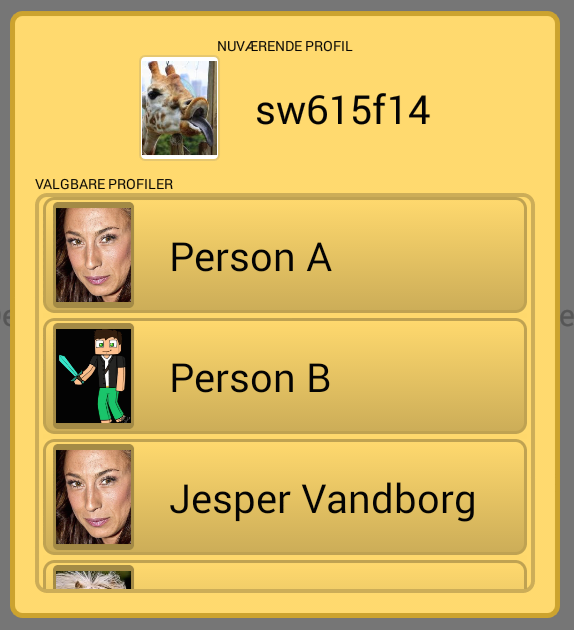
\includegraphics[width=0.55\textwidth]{sprint_three/puha_dialog}
        \caption{\androidinline{GProfileSelector}}
        \label{fig:puha_dialog}
\end{figure}

\FloatBarrier

This new component was implemented as a dialog by inheriting from the abstract dialog class from the components, called \androidinline{GirafDialog} (see \secref{sec:consistent_dialogs}). The functionality of this new profile selection dialog was to standardize the way the profile dialogs looks like, alongside functionality to allow the user to select either one or arbitrarily many profiles using this dialog.
\\\\
It was decided that profile pictures, using the \androidinline{PictogramItemView} component, should be displayed in a \androidinline{GridView} like seen in \figref{fig:dialog_profiles_selector}. The profiles in the grid should be clickable and allow the user to select the wanted profile easily. When a profile is selected, it is marked with a yellow color as indicator.

\begin{figure}[!htbp]
        \centering
        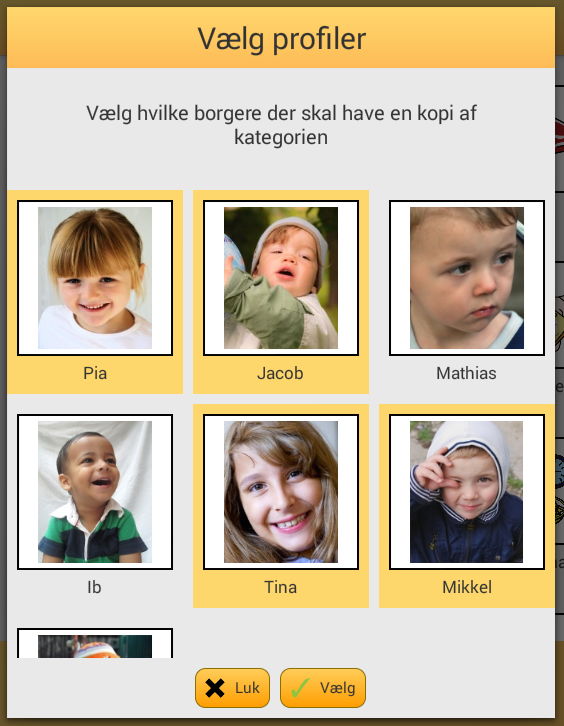
\includegraphics[width=0.55\textwidth]{sprint_three/dialog_profiles_selector}
        \caption{\androidinline{GirafProfileSelectorDialog}}
        \label{fig:dialog_profiles_selector}
\end{figure}

\FloatBarrier

It is also possible to set some profiles as marked upon opening the dialog for user selection. This was needed in the \ct for the functionality of administrating profiles and their categories. In case a category had been assigned to a citizen previously this citizen has been marked once the dialog reopens. When a guardian wants to assign, a category to a citizen the guardian must first create a category and then assign which citizens should have this category. In order to be consistent with the rest of the design, it was decided to implement the actual functionality to change profile and view it for a citizen as a button in the action bar. This rendered the ``Administrate Citizens'' button in the original design (see \secref{sec:home_screen}) useless, and it has therefore been removed. 